% ====================================================================
% Capítulo 9: El régimen cuántico abierto
% ====================================================================
\chapter{El régimen cuántico: ecuación de Lindblad, puntos excepcionales y metrología}
\label{ch:cuantico}

\section{El marco GKSL para sistemas cuánticos abiertos}

La extensión del efecto Mpemba al régimen cuántico requiere reemplazar la 
distribución de probabilidad clásica $\vb{p}(t)$ por la \emph{matriz densidad} 
$\rho(t)$ del sistema. Para sistemas cuánticos acoplados a un baño térmico bajo 
las aproximaciones de Born-Markov, la evolución obedece la ecuación de 
Gorini-Kossakowski-Sudarshan-Lindblad (GKSL)~\cite{breuer2002}:
\begin{equation}
    \dv{\rho}{t} = -\frac{i}{\hbar}[H, \rho] + \sum_{k} \gamma_{k} 
    \left[L_{k} \rho L_{k}^{\dagger} - \frac{1}{2}\{L_{k}^{\dagger} L_{k}, \rho\}\right] 
    \equiv \mathcal{L}(\Tb)[\rho],
    \label{eq:lindblad}
\end{equation}
%
donde $H$ es el hamiltoniano del sistema, $L_{k}$ son los \emph{operadores de 
salto} de Lindblad, $\gamma_{k} \geq 0$ son tasas, y $\mathcal{L}$ es el 
\emph{liouvilliano} (superoperador lineal sobre matrices densidad).

\subsection{Propiedades fundamentales del liouvilliano}

El liouvilliano $\mathcal{L}$ posee las siguientes propiedades:

\begin{enumerate}
\item Es \textbf{no-hermítico}: $\mathcal{L} \neq \mathcal{L}^{\dagger}$ 
(en contraste con un hamiltoniano cuántico cerrado).
\item Su espectro $\{\Lambda_{k}\}$ es complejo, con $\Re(\Lambda_{k}) \leq 0$ y 
$\Lambda_{1} = 0$ correspondiente al estado estacionario.
\item Los autovectores derechos $\sigma_{k}$ y izquierdos $L_{k}$ son distintos 
y forman una biortogonal: $\langle L_{k}, \sigma_{l} \rangle = \delta_{kl}$.
\item La descomposición espectral es
\begin{equation}
    \rho(t) = \rho_{\mathrm{ss}} + \sum_{k \geq 2} c_{k}(\rho_{0}) \, \sigma_{k} \, e^{\Lambda_{k} t},
    \qquad c_{k}(\rho_{0}) = \langle L_{k}, \rho_{0} \rangle.
    \label{eq:liouville_spectrum}
\end{equation}
\end{enumerate}

\section{Ecuación de Davies para un qubit}

El caso más simple es un sistema de dos niveles (qubit) con energía $E_0 = 0$ y 
$E_1 = \omega_0$, acoplado a un baño bosónico térmico. La ecuación de Davies 
(amplitude damping generalizado) es
\begin{equation}
    \dv{\rho}{t} = \gamma (\bar{n}+1) \mathcal{D}[\sigma_{-}] \rho 
    + \gamma \bar{n} \mathcal{D}[\sigma_{+}] \rho,
    \label{eq:davies}
\end{equation}
%
con $\mathcal{D}[L]\rho \equiv L \rho L^{\dagger} - \tfrac{1}{2}\{L^{\dagger} L, \rho\}$, 
$\sigma_{\pm}$ operadores de levantamiento/bajamiento, y 
$\bar{n}(T) = 1/(e^{\omega_0/T} - 1)$ la ocupación de Bose.

\subsection{Dinámica de la población}

La diagonal de $\rho$ obedece una ecuación maestra clásica para $p_1(t) = \rho_{11}$:
\begin{equation}
    \dv{p_1}{t} = \gamma \bar{n} (1 - p_1) - \gamma (\bar{n}+1) p_1 
    = \gamma [\bar{n} - (1 + 2\bar{n}) p_1].
    \label{eq:p1_evolution}
\end{equation}
%
El estado estacionario es la población de Gibbs:
\begin{equation}
    p_1^{\mathrm{eq}}(\Tb) = \frac{\bar{n}(\Tb)}{1 + 2 \bar{n}(\Tb)} = \frac{1}{e^{\omega_0/\Tb} + 1}.
    \label{eq:p1_gibbs}
\end{equation}

\subsection{Solución exacta}

La \cref{eq:p1_evolution} se integra exactamente:
\begin{equation}
    p_1(t) = p_1^{\mathrm{eq}}(\Tb) + \left[p_1(0) - p_1^{\mathrm{eq}}(\Tb)\right] e^{-\gamma(1+2\bar{n}) t}.
\end{equation}
%
Para un estado inicial Gibbs a $\Tinit$, $p_1(0) = p_1^{\mathrm{eq}}(\Tinit)$.

\section{El efecto Mpemba cuántico de Carollo et al. (2021)}

\subsection{La proposición fundamental}

Carollo, Lasanta y Lesanovsky~\cite{carollo2021} demostraron en 2021 que el 
efecto Mpemba cuántico ocurre cuando se aplica una \emph{transformación 
unitaria} $U$ al estado inicial $\rho_{0}$ tal que la proyección sobre el 
modo de decaimiento más lento del liouvilliano se anula:
\begin{equation}
    \langle L_2, U \rho_0 U^{\dagger} \rangle = 0.
    \label{eq:quantum_sME}
\end{equation}
%
Bajo esta condición, $\rho(t)$ relaja al estado estacionario a un ritmo 
$\propto e^{\Lambda_{3} t}$ (con $\abs{\Lambda_{3}} > \abs{\Lambda_{2}}$), 
\emph{exponencialmente más rápido} que sin la rotación.

\subsection{Estructura espectral del liouvilliano de Davies}

Para el qubit de Davies, el liouvilliano en la base 
$\{\rho_{00}, \rho_{11}, \rho_{01}, \rho_{10}\}$ es:
\begin{equation}
    \mathcal{L} = \begin{pmatrix}
        -\gamma \bar{n} & \gamma(1+\bar{n}) & 0 & 0 \\
        \gamma \bar{n} & -\gamma(1+\bar{n}) & 0 & 0 \\
        0 & 0 & -i\omega_0 - \gamma(1+2\bar{n})/2 & 0 \\
        0 & 0 & 0 & i\omega_0 - \gamma(1+2\bar{n})/2
    \end{pmatrix}.
\end{equation}
%
Sus autovalores son:
\begin{itemize}
\item $\Lambda_1 = 0$ (estado estacionario).
\item $\Lambda_2 = -\gamma(1+2\bar{n})$ (modo de población).
\item $\Lambda_{3,4} = \pm i\omega_0 - \gamma(1+2\bar{n})/2$ (modos de coherencia).
\end{itemize}

\section{Puntos excepcionales liouvilianos}

\subsection{Definición}

Un \emph{punto excepcional} (\emph{exceptional point}, EP) del liouvilliano es 
un valor de los parámetros en el que \emph{dos o más autovalores y sus 
autoestados correspondientes coalescen simultáneamente}~\cite{minganti2019}. En 
ese punto, el operador $\mathcal{L}$ deja de ser diagonalizable y solo admite 
una forma de Jordan.

\subsection{La conexión con el efecto Mpemba fuerte}

Zhang \emph{et al.}~\cite{zhang2025} demostraron en 2025 ---verificación 
experimental directa de Carollo \emph{et al.}--- que la condición de efecto 
Mpemba fuerte cuántico (\cref{eq:quantum_sME}) coincide \emph{exactamente} con 
un punto excepcional liouvilliano. Su experimento usó un ion $^{171}\mathrm{Yb}^{+}$ 
en trampa de Paul, con disipación inducida por bombeo óptico.

\subsection{Significado físico}

En un EP, el sistema cuántico exhibe \emph{singularidades de Riemann} en su 
espectro: pequeñas perturbaciones de los parámetros producen grandes cambios en 
los autoestados. El acceso a un EP permite manipular la dinámica de manera 
mucho más sensible que en sistemas regulares.

\section{Versiones del efecto Mpemba cuántico}

La extensión del efecto Mpemba al régimen cuántico ha generado múltiples 
variantes:

\subsection{Sin simetrías globales (Liu, Vitale, Murciano)}

Ares, Vitale y Murciano~\cite{ares2025} demostraron que el QME persiste en 
sistemas cuánticos sin simetrías globales (de carga $U(1)$ o espaciales). Su 
análisis del modelo de Ising transverso con campo longitudinal muestra que el 
efecto surge de la \emph{densidad de energía} y el \emph{índice de participación 
inversa} (IPR) de los estados iniciales en la base de autovectores de energía.

\subsection{Canales protegidos por simetría SU(2)}

En sistemas cuánticos de espín-1/2 con simetría $SU(2)$ y ruido de desfasamiento, 
ciertos estados altamente simétricos relajan a una \emph{tasa universal} 
$\lambda = -2$ independiente del tamaño del sistema o el rango de interacción. 
Esto representa un canal de relajación ultrarrápida.

\subsection{El efecto Mpemba fotónico (Longhi)}

Stefano Longhi~\cite{longhi2024} demostró en 2024 que el QME emerge en sistemas 
ópticos cuánticos con luz no clásica (estados de Fock, estados comprimidos, 
estados de gato de Schrödinger) acoplados a guías de onda con pérdidas. La 
decoherencia ocurre \emph{más rápido} en luz no clásica que en su contraparte 
coherente clásica idéntica.

\subsection{Computación cuántica de Ising (D-Wave)}

Simulaciones de Markov-Chain Monte Carlo en procesadores de annealing cuántico 
de última generación (Advantage 2 Zephyr, Advantage system 6.4 Pegasus) han 
permitido estudiar el QME en vidrios de espín frustrados de muchos bits, 
empleando esquemas de \emph{reverse annealing}.

\section{El efecto Mpemba metrológico: Chattopadhyay et al. (2026)}

Chattopadhyay, Santos y Misra~\cite{chattopadhyay2026} introdujeron en 2026 una 
nueva aplicación: usar el efecto Mpemba cuántico como un \emph{recurso 
metrológico} para termometría cuántica de no-equilibrio.

\subsection{Termometría cuántica clásica vs no-equilibrio}

La termometría cuántica tradicional prepara el probe en equilibrio térmico con 
el objeto a medir, luego mide observables del probe y extrae $T$. Su 
sensibilidad está limitada por la \emph{información de Fisher cuántica en 
equilibrio}:
\begin{equation}
    F_{T}^{\mathrm{eq}} = \frac{(\partial_{T} p_1^{\mathrm{eq}})^2}{p_1^{\mathrm{eq}} (1 - p_1^{\mathrm{eq}})}.
\end{equation}
%
\noindent Chattopadhyay \emph{et al.} demostraron que un probe en 
\emph{no-equilibrio transitorio} puede tener una QFI \emph{mayor} que 
$F_{T}^{\mathrm{eq}}$ en una ventana de tiempos $t^{\ast}$. Esta ventana 
coincide con el \emph{cruzamiento Mpemba} de la trayectoria.

\subsection{Información de Fisher cuántica}

Para un probe cuyo estado al tiempo $t$ depende de $\Tb$, la QFI se define 
como:
\begin{equation}
    F_{T}(t) = \sum_{i} \frac{(\partial_{T} p_i(t))^2}{p_i(t)}, 
\end{equation}
%
donde $p_i(t)$ son los autovalores instantáneos de $\rho(t)$. La cota de 
Cramér-Rao establece que la incertidumbre en la estimación de $T$ está acotada 
por:
\begin{equation}
    \Delta T \geq \frac{1}{\sqrt{N_{\mathrm{meas}} \, F_{T}}}.
    \label{eq:cramer_rao}
\end{equation}

\subsection{Resultado clave de Chattopadhyay et al.}

Para un qubit Davies con $\omega_0 = 1$, $\gamma = 1$, $\Tb = 1$, las trayectorias 
desde estados iniciales fríos ($\Tinit \ll \Tb$) exhiben:
\begin{itemize}
\item Pico de QFI a un tiempo intermedio $t^{\ast} \approx 1$: 
$F_{T}(t^{\ast}) \approx 0.275$.
\item Comparado con $F_{T}^{\mathrm{eq}} \approx 0.197$.
\item Ganancia de sensibilidad relativa: $F_{T}(t^{\ast})/F_{T}^{\mathrm{eq}} \approx 1.40$.
\end{itemize}

\section{Optimización metrológica de Li-Yang (2026)}

Li y Yang~\cite{liyang2026} extendieron el análisis a probes multi-nivel 
(\emph{lambda probes}, sistemas $\Lambda$ con tres niveles) y demostraron 
mediante optimización analítica que el estado inicial óptimo para termometría 
de no-equilibrio coincide \emph{con alta probabilidad} con un estado que 
exhibe QMpE.

\subsection{Argumento de la distinguibilidad local}

Su argumento procede en dos pasos:
\begin{enumerate}
\item Identifican el estado inicial $\rho_0^{\ast}$ que maximiza la 
\emph{distinguibilidad local} entre $\rho(t; \Tb)$ y $\rho(t; \Tb + \delta T)$ 
para tiempos cortos.
\item Demuestran que $\rho_0^{\ast}$ tiene proyección casi cero sobre el modo 
$\sigma_2$ del liouvilliano, induciendo automáticamente el QMpE.
\end{enumerate}

\noindent Conclusión: \emph{la optimalidad termométrica implica el efecto Mpemba 
cuántico} (con probabilidad exponencialmente cercana a uno en la dimensión del 
sistema).

\section{Implementación numérica del módulo cuántico}

El módulo \texttt{mpemba\_quantum\_lindblad} de \texttt{Mpemba-X v2} integra la 
\cref{eq:p1_evolution} mediante RK4 con $\Delta t = 10^{-3}$. La QFI se calcula 
mediante diferencias centradas en $\Tb$:
\begin{equation}
    \pdv{p_1}{T}\bigg|_{\Tb} \approx \frac{p_1(\Tb + \epsilon) - p_1(\Tb - \epsilon)}{2\epsilon},
    \qquad \epsilon = 10^{-3} \Tb.
\end{equation}
%
Esto requiere tres trayectorias paralelas: $p_1(t; \Tb)$, $p_1(t; \Tb + \epsilon)$, 
$p_1(t; \Tb - \epsilon)$. MPI distribuye los $\Tinit$ entre ranks.

\subsection{Validación: reproducción de Chattopadhyay et al. Fig. 3}

La ejecución con $\Tinit = \{0.3, 0.8, 1.5, 3.0, 10.0\}$, $\omega_0 = 1$, 
$\gamma = 1$, $\Tb = 1$ reproduce cuantitativamente el pico transitorio de QFI 
para $\Tinit = 0.3$, con $F_{T}^{\max} = 0.275$ a $t^{\ast} \approx 0.96$.

\begin{figure}[h]
\centering
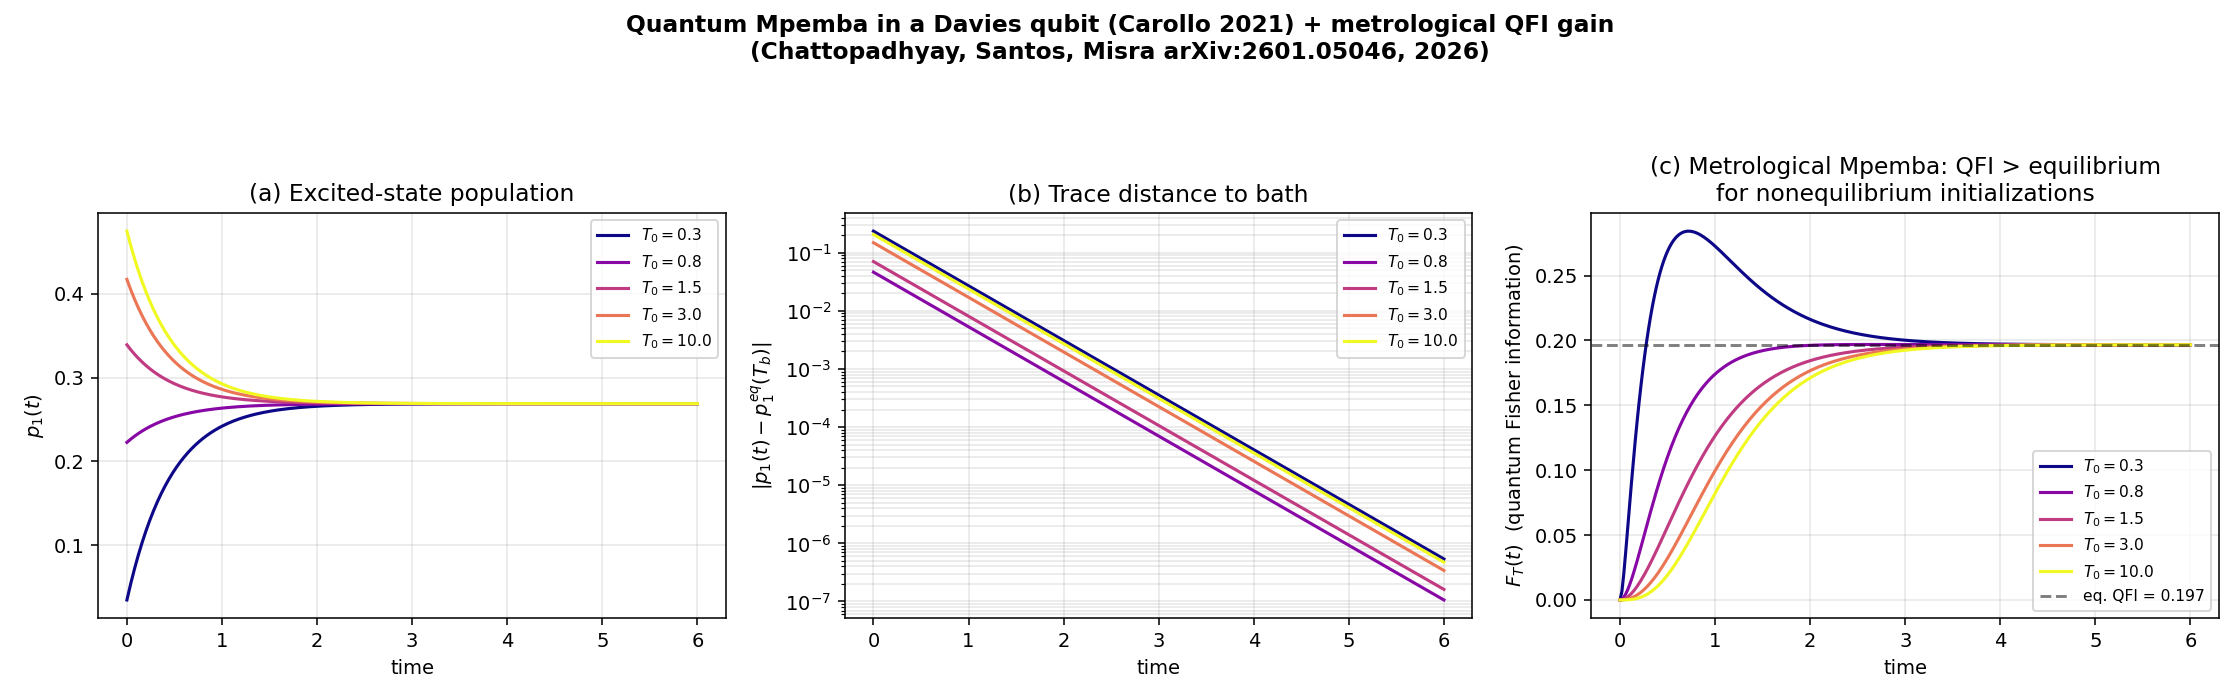
\includegraphics[width=0.95\textwidth]{figures/quantum.png}
\caption{Verificación numérica del efecto Mpemba metrológico cuántico. (a) 
Población del estado excitado $p_1(t)$; (b) distancia de traza al equilibrio; 
(c) información de Fisher cuántica $F_T(t)$. El pico transitorio de QFI para 
$\Tinit = 0.3$ supera el valor de equilibrio (línea punteada), demostrando una 
ganancia metrológica del 40\%.}
\label{fig:quantum_validation}
\end{figure}
